\documentclass[output=paper]{langsci/langscibook} 
\author{Alexander M. Teixeira Kalkhoff\affiliation{Universität Regensburg}}
\title{Using corpus data for testing a working hypothesis about Haitian Creole prosody}
\shorttitlerunninghead{Using corpus data for testing a hypothesis about Haitian Creole prosody}
% \chapterDOI{} %will be filled in at production

\abstract{The goal of the corpus-based study in hand is to gather information about Haitian Creole prosody, i.e. prosodic constituency and the location and nature of prosodic events within utterances, and to assess the working hypothesis of a hybrid prosodic system exploring the linguistic resources of the {Corpus of Northern Haitian Creole} freely accessible online. The main concerns are technical and methodological aspects of creole language prosody research, such as automatic audio–text alignment and segmentation of the signal, annotation in Praat, recording and interview settings, and, of course, the linguistic interpretation of the observed prosodic phenomena.
}

% {Keywords:} Haitian Creole, prosody, hybrid prosodic system hypothesis, corpus-based.

\maketitle



\begin{document}
\label{chap:kal}
\section{Introduction}

Haitian Creole (henceforth HC) is a sociohistorical and linguistically well-described creole language (\citealt{Fattier2013,Valdman2014}, see there for related references). However, to date, the majority of relevant linguistic descriptions have focused on the grammar and the lexicon. There are only a few studies about HC prosody and intonation. That reflects a general tendency, which is doubtlessly due to methodological problems and the complexity of describing prosodic features and intonational patterns (see, for example, \textit{The Atlas of Pidgin and Creole Language Structure} 2013, which contains only three chapters on the prosodic level, namely on syllables and tones). Nevertheless, there are some very interesting relevant investigations, such as \citet{Hualde2008palenquero}, investigating intonation in Palenquero, and Shelome \citet{Gooden2014}, establishing an intonational phonology of Jamaican Creole.

The Indiana University Creole Institute provides the freely available \textit{Corpus of Northern Haitian Creole} online, a corpus of ten hours of spoken HC speech data. The main goal of my contribution is to show how one can use this valuable speech resource to hypothesize and test prosodic features of spoken HC. However, since the technical aspect of the corpus is rudimentary, the editing task was twofold. Firstly, the quality of the audio files had to be assessed, stabilized, and, where applicable, improved for further phonetic and prosodic analyses. Secondly, a sound–text alignment and word-and-segment-sized segmentation had to be accomplished automatically by using tools and services provided openly and free of charge for researchers by the \textit{Bavarian Archive for Speech Signals} (BAS). BAS is part of the CLARIN-D (\textit{Common Language Resources and Technology Infrastructure}) research infrastructure for humanities and social sciences (\url{http://www.clarin-d.de}). 

The goal was to establish the workflow for prosodic analysis in Praat (\citealt{Boersma.praat}) in order to scrutinize both relevant prosodic constituents and the location and nature of prosodic events within those constituents.

The paper is organized as follows. In \sectref{sec:kal:2}, I will expose a working hypothesis according to which HC is characterized by a hybrid prosodic system shaped by influences from West African languages and French. \sectref{sec:kal:3} describes how to establish the workflow for a ten-minute test piece for prosodic annotation and analysis using the technically deficient means of the \textit{Corpus of Northern Haitian Creole}. Based on that short corpus fragment, \sectref{sec:kal:4} discusses some prosodic features of HC and reconsiders the working hypothesis. \sectref{sec:kal:5} discusses the pros and cons of a corpus-based approach to HC prosody and intonation. Finally, \sectref{sec:kal:6} sums up the results.


\section{\label{sec:kal:2} Working hypothesis: Haitian Creole prosody as a hybrid prosodic system}

Besides the technical aspects of the corpus-based approach, I had to establish a working hypothesis about the prosodic system of HC as a starting point for my research, because, as mentioned above, HC is a grammatically and lexically well-described language, but only limited information is available about its prosodic and intonational nature (\citealt{Cadely1997,Brousseau2003,Fattier2005}). Please note that in what follows, I will focus on prosodic features, such as prosodic constituency, accentuation patterns, tones, and so on. HC intonation, which relates to illocution and information structuring, I will disregard here.

HC genesis took place in Saint-Domingue, the western part of the Caribbean Hispaniola Island, within the sociohistorical context of slave trade and plantation society (\citealt{McWhorter2005,Eltis2010}). In the late 17\textsuperscript{th} century, French colonialists started to buy West African slaves for their growing sugar plantations. Thus, linguistic sources for the HC genesis are French as the major lexifier language (superstratum), languages from the Kwa group of West Africa, especially Gbe, Bantu languages of Central Africa (both groups as substratum), and some influences of Spanish, English, and Amerindian languages (e.g. Arawak-Taíno, Tupi) (\citealt[52-57]{Lefebvre2006}; \citealt[195]{Fattier2013}). Researchers acknowledge a large predominance of the West African Gbe languages.

While the origin of the HC lexicon is traditionally linked to French and the origin of HC grammar to West and Central African substratum languages, there is no clear statement about the origin of HC prosody. According to Shelome Gooden and her colleagues’ model of a “hybrid prosodic system” for Jamaican Creole (\citealt{Gooden2009}, see there for related references), I argue also for a hybrid prosodic system for HC that is shaped by both French and the West African substratum languages (for a similar approach see \citealt{Brousseau2003}).

Aware that I talk about linguistic events in the past, which started around 1700, and that prosodic systems may evolve like the grammar or the lexicon of a given language, I am using for heuristic reasons synchronic accounts of French and West African languages for lack of diachronic information. Since I am analyzing contemporary HC, which is still in language contact with today’s French and West African languages, I assume that that heuristic is admissible.

Typologically, linguists consider the French prosodic system as a stress accent system \citep{Hyman2006}. French is supposed to have not word accent, but a phrase accent (\citealt[460]{Hulstetal2010}). Its prosodic constituents, i.e. the hierarchized domains of prosodic events, are Intonational Phrase (IP), Intermediate Phrase (ip), and Accent Phrase (AP) (for the most recent account of the prosodic constituency and intonational phonology of French see \citealt{Delais-Roussarie2015}, see there for related references). An AP contains one or more content words accompanied by its/their functional words; the IP contains one or more APs; and the status of the intermediate constituent ip is controversial. The most influential prosodic domain in French is the AP with its facultative left initial phrase accent and its obligatory right pitch accent because – contrary to the prosodic hierarchy – the AP governs the pitch accent of the superordinate IP (\citealt{Jun2000,Jun2002}; \citealt[76]{Delais-Roussarie2015}). 

Since, as mentioned above, French does not have word accent, i.e. a lexically distinctive fixed syllable-related pitch movement within words, researchers discuss controversially the status of observable pitch movements within phonological phrases and utterances. \citet{Jun2002}, for instance, advocate a facultative positionally free initial phrasal accent on the left and an obligatory positionally fixed pitch accent on the right edge of the AP. Without doubt, the most salient prosodic event in French happens on the stressed last full syllable on the right edge of the IP. Speakers of French realize phonetically this primary stress by cumulative means of lengthening, articulatory strengthening (\citealt{Fougeron1997}), and pitch movement, although the lengthening is the most salient one. Hence, the specific rhythm of French results from the alternation or a-isochrony of lengthened and short syllables \citep{Dufter2004}. As other Romance languages, French is classified as a \textit{syllable timed language}, or, more adequately, as a \textit{syllable language} \citep{Auer2001}.

West African prosodic systems are considered typologically as tone systems (\citealt{Creissels1997,Hyman.2001,Hyman2006}, \citealt[381-427]{Hulstetal2010}). We can distinguish between lexical, grammatical, and pragmatical tones. Lexical tones are lexically distinctive syllable/mora-specific pitch movements within words \citep{Yip2002}. Grammatical tones mark function word classes or morphemes and pragmatical tones mark focus (for Ewe see \citealt[133-202]{Stahlke1971} and \citealt{Fiedler.2013}). Intonationally, West African languages are characterized as “terrace-level languages”, that is a terrace-shaped downward trend in pitch visualizations. In summary, linguists characterize them as poor in intonation (\citealt{Welmers1959,Kuegler.2016Akan}).

Doubtlessly, the most striking prosodic features of this listing are the primary stress at the right edge of the IP for French and the tones for West African languages. I will pay special attention to these two prosodic features while examining HC prosody, expecting some traces from the contributing prosodic systems assuming the working hypothesis of hybrid systems. 

That finally leads to the questions: What are the prosodic features of HC? What are the prosodic units of HC? Which part of the prosodic unit can be stressed? By which phonetic means? 

In the corresponding research literature, \citegen{Brousseau2003} investigation is the most exhaustive study of HC prosody. Beyond that, I could only find a few scattered hints (highlighted by the author):  \citet[140-149]{Dejean1980} mentions the \textit{clitic group} as domain of external sandhi.  \citet[5]{Valdman1988} highlights emphatic words to place emphasis on a particular word, because Haitian Creole \textit{does not have word stress}. According to the hybrid nature of HC prosody, \citet[123]{Brousseau2003} concludes that HC “is a \textit{stress system} (like French), realized at the level of \textit{phonological word} (like Fongbe) and \textit{quantity sensitive} (unlike French or Fongbe)”.  \citet[196]{Fattier2013} mentions a “\textit{fixed word stress on the last syllable} of the word”.  As we can see, there are some conflicting statements, for example about the HC word stress. 

However, before scrutinizing prosodic features of HC, I had to manipulate corpus data from the \textit{Corpus of Northern Haitian Creole} to establish a workflow for prosodic annotation and analysis in Praat.


\section{\label{sec:kal:3}Establishing the workflow for prosodic analysis}
\subsection{The Corpus of Northern Haitian Creole}
 
Recorded in 2007 and subsequently published by the Indiana University Creole Institute under the auspices of Albert Valdman, the \textit{Corpus of Northern Haitian Creole} nowadays constitutes a freely available and downloadable online resource for linguistic research on HC \citep{Valdman.corpus}. It documents speakers of Capois, i.e. the language variety of HC spoken in the north of Haiti near Cap Haïtien. The mentioned webpage gives access to the audio files of the recordings, to the text files of the transcripts, and to the transcription conventions of ten interviews of altogether approximately ten hours of speech data. Audio files are saved as MP3 and the transcripts as Microsoft® Word files with an overall size of 509 MB. 

Beyond doubt, the gravest technical problem for further prosodic analysis is that the recordings were saved in the lossy compressed MP3 (MPEG-1 Audio Layer 3) audio format (128 kBit per second, 44.1 kHz) instead of WAV (Waveform Audio File Format) (1411 kBit per second, 44.1 kHz) or another lossless audio format. Unfortunately, even at the Indiana University Creole Institute there are no lossless compressed or uncompressed original recordings available, as I learned on inquiry. It implies that some parts of the physical sound signal are irrecoverably lost. This is a fact that must stay in mind, for example, while interpreting the fundamental frequency movements for tone assignment, because phonetic analysis tools, such as Praat, have difficulties computing fundamental frequency starting from a lossy sound signal. Another phonetic factor that may interact with the algorithms of automatic pitch computing is the noisy background of the field recordings, e.g. other voices, birds or tools, due to the environment of the interview sessions, to a greater or lesser extent. For that reason, interview numbers 5, 6, 7, 8, and 10, altogether 50\% of the corpus data, cannot be used at all for prosodic analysis.

Another technical concern is that there is no link between the audio and text files. However, we need such a temporal alignment for the interpretation of phonetic events relative to what is said. As we will see later, this alignment task will be accomplished automatically by using the MAUS (Munich AUtomatic Segmentation) tool developed and provided by the \textit{Bavarian Archive of Speech Signals} \citep{Schiel1999,kisler2017MAUS}. However, first, I had to resolve another problem: Because there are no separate audio tracks (or audio channels) for each speaker, as is necessary for the automatic sound–text alignment, I had to segment the turns of each speaker manually using a Praat text grid. 

Finally, yet importantly, nobody translated the transcripts from Capois to French or English, which makes the direct access to the meaning of the HC speech data difficult. Therefore, I had to translate relevant text passages by myself.

Even though the initial material conditions of the \textit{Corpus of Northern Haitian Creole} do not really favor prosodic and intonational research, the following subsection will show how I established the workflow for a test run. The ultimate goal of this editing process was to use speech data from the corpus for prosodic analysis in Praat. 

\subsection{Editing a test piece}
To establish the workflow for the test run, I chose a ten-minute test piece from the first interview. Interview 1 has a total length of 1 hour and 12 minutes. Selection criteria were, first, the selected test piece should not be too close to the beginning nor to the end of the interview, because a more natural and relaxed social and linguistic interaction between the speakers was expected after a certain time of contact and the fading of the awareness of being recorded. Second, the test piece should include some turn takings and longer turns of one speaker to get some impressions of intonational variation by contrast and prosodic/intonational shape of the utterance by one speaker at the same time. Third, the test piece should start and end with complete turns. 

The first step of the editing process, choosing and editing a ten-minute test piece of the audio signal, I executed with the open-source freeware Audacity® (version 2.0.6), freely available software for high-quality recording and sound editing \citep{AudacityTeam}.\footnote{According to my selection criteria, I chose the ten-minute audio piece within the time interval from 00h19min25.800sec to 00h29min23.000sec of interview number 1, which corresponds to lines 211 to 332 of the transcript.} To level the different volumes of the speakers’ voices within the audio signal, caused, for instance, by different distances to the recording device, I used the automatic normalization function of Audacity®. The outcome of the normalization procedure is a smoothed audio signal with regard to changes in volume.

As mentioned above, a general problem of field recordings are the sometimes considerable background noises. My ten-minute test piece was concerned with a constant cricket noise in the background. To reduce that unwanted noise, assuming that it would interfere with the automatic phonetic analysis with Praat, I executed the denoising procedure implemented in Audacity®. Effectively, the procedure reduced the cricket noise, but also further damaged the physical sound signal. Linguists should keep in mind that every damaging treatment of the sound signal, such as compressing to MP3 or denoising, could perturb or hamper automatic segmentation and alignment processes or Praat algorithms. As we will see below, the MAUS algorithm was robust enough to segment and align the denoised sound signal of my test piece.

To avoid further damage of the sound signal by continuing to save as MP3 – every saving as MP3 causes new data loss – the test piece was saved as WAV audio file, while, of course, the first and fundamental damaging resulting from MP3 compression persists. It is important to note that blanks within the file name have to be avoided for further untroubled use with Praat and the BAS tools.

The second step for my test run was to prepare the corpus data for the automatic sound–text alignment and word-and-segment-sized segmentation tools provided by the \textit{Bavarian Archive of Speech Signals} \citep{kisler2017MAUS}. The specificity of my case was that MAUS and WebMAUS \citep{Kisler2012} and the underlying Grapheme-to-phoneme converter \citep{Reichel.2012} has been run for many other languages, such as English, German, French, Italian, Hungarian, and Russian, but until now not for HC. My trump was that HC orthography is phonemic, so that the prognosis that MAUS will also run for HC was quite favorable; I will explain that with more details later. 

First, I had to edit the piece of transcript by removing all metalinguistic information, because MAUS would interpret them as something that is said in the conversation and thus confuse the automatic alignment procedure. So, the “XXX” sign standing for unintelligible parts within the audio signal was replaced by the MAUS placeholder category “<nib>”. All extralinguistic information, such as “(rire)” ('to laugh'), all typographical features, such as underscores, bold face type, and ellipsis, and all additional standard HC orthography remarks, such as the second “(paske)” in “pase (paske)” ('because'), were removed. Superscript letters were pulled down, such as in “sè\textsuperscript{r}vi”, which became “sèrvi” (for more details about the meaning of used metalinguistic information within the transcript see the transcription conventions of the corpus on its website). The MAUS category “<p:>” standing for longer pauses also improves the later alignment and segmentation procedure.

Because there are three speakers, two consultants (“R” and “S” in the transcript) and the interviewer (“K” in the transcript), but no distinct audio channels for each of them, I had to perform the so-called chunk segmentation manually. If I had not done that, MAUS would not have known who is speaking in a given moment in the interview and interpret the data from the audio signal as one sole turn. In addition to that, no acoustic model of MAUS contains pauses longer than 3 sec. Therefore, without chunk segmentation that also includes pause information, the MAUS segmentation procedure would set segment boundaries misleadingly within longer breaks. The chunk segmentation procedure consists in the creation of a *.TextGrid annotation file using Praat with three interval annotation tiers, namely R, S, and K for each speaker. At the starting and end point, I set a boundary and filled in the adjusted text from the transcript. Praat converts the text automatically from the *.doc into the appropriate *.txt format. I saved the text grid file.

In sum, the manual chunk segmentation is quite time-consuming, particularly if we consider a bigger amount of speech data. For the output of our chunk segmentation in Praat, see \figref{fig:kal:1}.

\begin{figure}
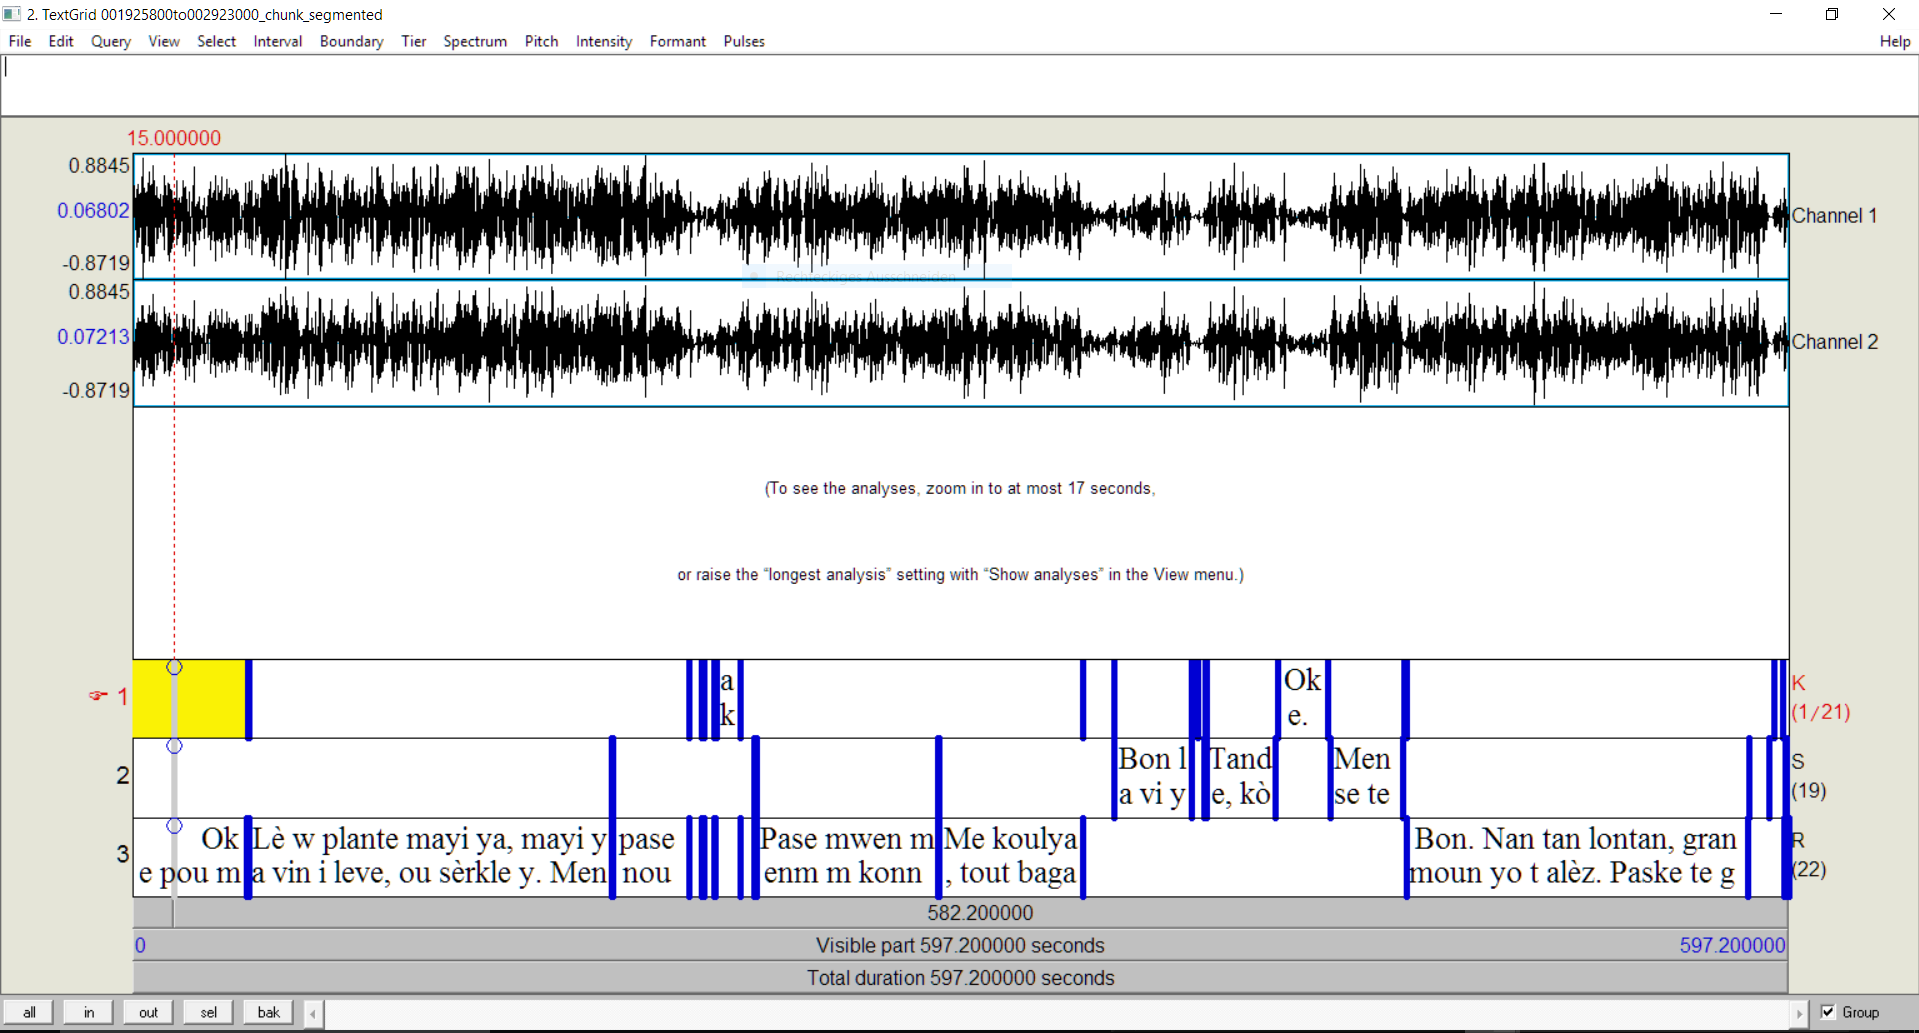
\includegraphics[width=\textwidth]{figures/KALPeerreviewedkorr-img1.png}
\caption{\label{fig:kal:1} Output of the manual chunk segmentation procedure.}
\end{figure}

Since the BAS tools had previously never been ran for HC, the BAS team had to modify them. First, they chose “extended German” as the underlying acoustic model for the later HC segmentation and alignment. The reason for this was twofold: Firstly, there is a wide congruence of the German and HC phoneme inventory and, secondly, the MAUS algorithm was trained extensively with German but not, for example, with French speech data. Therefore, the expectation was that the German acoustic model would work more reliably for the forced alignment procedure of the HC transcript data with the acoustic signal.

As mentioned above, the advantage of the HC orthography is its phonemic nature, i.e. there is a tight relationship between the established spelling system and pronunciation (for more details about HC orthography see \citealt[x-xiii]{Valdman1981}). Let us compare, for example, HC <konba> with French <combat> [k[F08D?][F029?]ba] (combat-\textsc{n.sg}), where HC <on> regularly indicates nasalized \textit{o} and the unpronounced final \textit{t} does not appear orthographically in contrast to French. Another more striking example is HC <mwa> compared to French <mois> [mwa] (month-\textsc{n.sg}), where today’s French orthography does not reflect the present pronunciation at all, while the HC spelling does. Consequently, all HC alphabetic characters represent sounds, whereas the French etymological orthography carries many phonetically empty characters pronounced only in the past.

The BAS team prepared and executed the MAUS text alignment and segmentation procedure of the chosen corpus data. On inquiry, they gave some background information that can be helpful to replicate the procedure for similar purposes. The whole procedure contained three steps: (i) chunk preparation, (ii) grapheme–phoneme conversion, and (iii) signal–text alignment.

(Ad i) To prepare the chunks for the grapheme–phoneme conversion and the signal–text alignment, they transformed the Praat text grids from my manual turn segmentations into three BAS Partitur Format files, one for each speaker.\footnote{\url{https://www.phonetik.uni-muenchen.de/Bas/BasFormatseng.html\#Partitur}} This step was carried out by means of the BAS web service “Chunk Preparation”.\footnote{\url{http://clarin.phonetik.uni-muenchen.de/BASWebServices/\#/services/ChunkPreparation}\\ Service options (deviating from defaults): Language: Haitian Creole; Input format: tg; Input tier name: {<}name of the respective chunk tier in the TextGrid{>}; Sampling rate: 44100.} Each of these BAS Partitur files contains two tiers: ORT for the orthographic words and TRN for the time (onset and length) information of the chunks. 

(Ad ii) For the grapheme–phoneme conversion, they handcrafted a grapheme–phoneme mapping table, which maps HC letter sequences to extended German SAM-PA (\textit{Speech Assessment Methods Phonetic Alphabet}) including nasal vowels. To each of the BAS Partitur files they added a KAN tier using the BAS web service “Grapheme2Phoneme”.\footnote{\url{http://clarin.phonetik.uni-muenchen.de/BASWebServices/\#/services/Grapheme2Phoneme}} The KAN tier contains the canonical transcription of each word derived by means of greedy mapping, which means the longest letter sequence first, looked up in the handcrafted mapping table.\footnote{Service options (deviating from defaults): Language: Haitian Creole; Input format: bpf; Sampling rate: 44100; Output Symbol inventory: sampa; Output format: bpf; Tool embedding: maus.}

(Ad iii) The BAS web service “WebMAUSGeneral”\footnote{\url{http://clarin.phonetik.uni-muenchen.de/BASWebServices/\#/services/WebMAUSGeneral}} added to each of the BAS Partitur files a MAU tier. Due to the model language mismatch, the HC segmentation ran in the forced-alignment mode, which means that MAUS aligned the entire canonic transcription to the audio signal ignoring spontaneous speech phenomena.\footnote{Service options (deviating from defaults): Language: German, Output format: TextGrid; KAN tier in TextGrid: true; ORT tier in TextGrid: true; Chunk segmentation: true // make use of TRN tier; MAUS modus: align // forced alignment.} In contrast, for trained acoustic models, such as German or English, the MAUS algorithm calculates a huge variance space of possible variants of pronunciation together with their probability based on the canonical pronunciation. MAUS searches that variance space while aligning the orthographic text from the transcript to the real acoustic signal, which can represent considerable phonetic variance compared to the calculated standard pronunciation. 

The output format of the MAUS procedure is a Praat text grid for each of our three speakers containing the interval tiers ORT, standing for word-tokenized orthographic transcript, KAN, standing for canonical pronunciation, and MAU, standing for SAM-PA encoded phonemes; see \figref{fig:kal:2}. I saved the three text grids.

\begin{figure}  
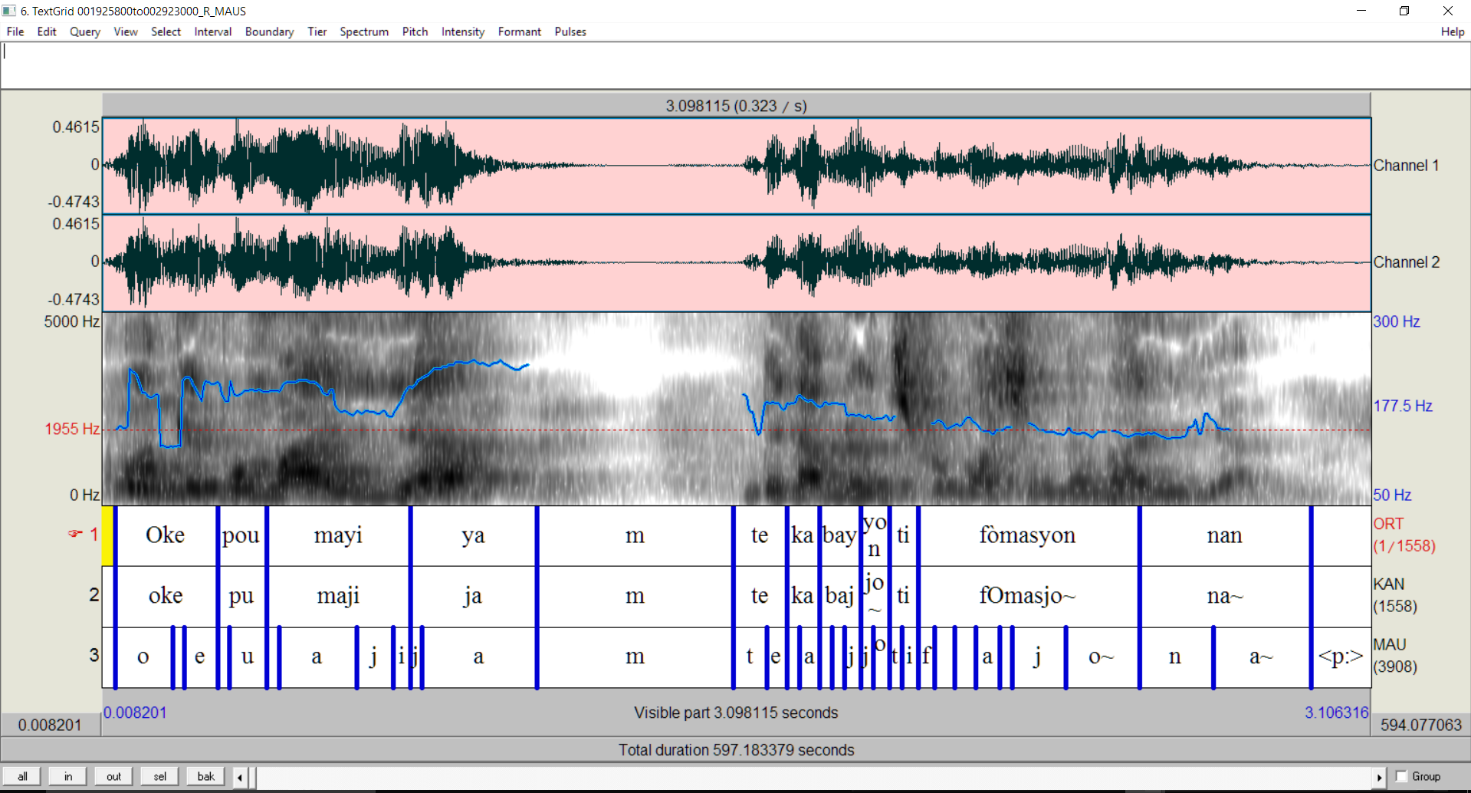
\includegraphics[width=\textwidth]{figures/KALPeerreviewedkorr-img2.png}
\caption{\label{fig:kal:2} Example of the output of the MAUS procedure for speaker R.}
\end{figure}


As we can see in \figref{fig:kal:2}, the edited piece of the audio file together with the text grid from the MAUS procedure calculated from the transcript generate the desired output in Praat as the base for later prosodic annotation and analysis. The text is aligned with the sound signal, the text is word-and-segment-sized segmented, and Praat could perform the automatic pitch analysis “Sound: To Pitch…” (autocorrelation). For the pitch contour view, the pitch range between 50 and 300 Hz (“Advanced pitch settings”) was chosen. Nevertheless, we have to keep in mind that the initial sound signal from the corpus has been damaged by saving as MP3 and denoising. Therefore, the calculation of the pitch contour in Praat can suffer from complications. Hence, a permanent comparison of the calculated pitch contour with the first harmonic from the spectrogram should be mandatory.

\subsection{Prosodic annotation}
To annotate prosodically the test piece in Praat \citep{Boersma.praat}, I established the following annotation tier hierarchy using the MAUS output text grids: (1) ORT for the orthographic words from the transcript as an interval tier, (2) MAU for SAM-PA encoded segments as an interval tier as well, (3) BIN for break indices as a point tier, (4) TON for a first descriptive phonetic tonal assignment using ToBI tone labels as a point tier, (5) TRA for word-by-word translation into English and grammatical glossing as an interval tier, and (6), (7), and (8) K, S, R for the chunk-segmented turns of the three speakers K, S, and R as interval tiers. Praat allows the extraction and merging of annotation tiers from different text grids (“Extract one tier” and “Merge” Praat functions). The newly merged text grid was saved.

The break index question concerns the prosodic structure of a given language. For HC I assume the crosslinguistically attested prosodic hierarchy of Intonational Phrase < Intermediate Phrase < Accentual Phrase/clitic group < prosodic word (for more details and references see the next subsection). Consequently, the break index BI 4 indicates Intonational Phrase boundaries, BI 3 indicates Intermediate Phrase boundaries, BI 2 indicates clitic group boundaries, BI 1 indicates prosodic word boundaries, and BI 0 indicates function word junctures.

The main concerns of the annotation process were the readjustment of some boundaries, the identification of prosodic constituents and the respective break index assignment, the labelling of salient tonal movements, and translation and glossing. For that first phonetic tonal assignment I used ToBI labels such as H, L, LH, H\%, L\%, and so on (\citealt{Silverman1992,BeckmanAyers1994,Beckman2005}) (for the outcome of the annotation process see the example in \figref{fig:kal:3}). Of course, at this point of my analysis, the results are purely descriptive. My focus was to identify the location and nature of prosodic events, not to establish an intonational phonology of HC, which remains a goal for further research. Neither was my annotation crosschecked by any intertranscriber reliability test.

\begin{figure}  
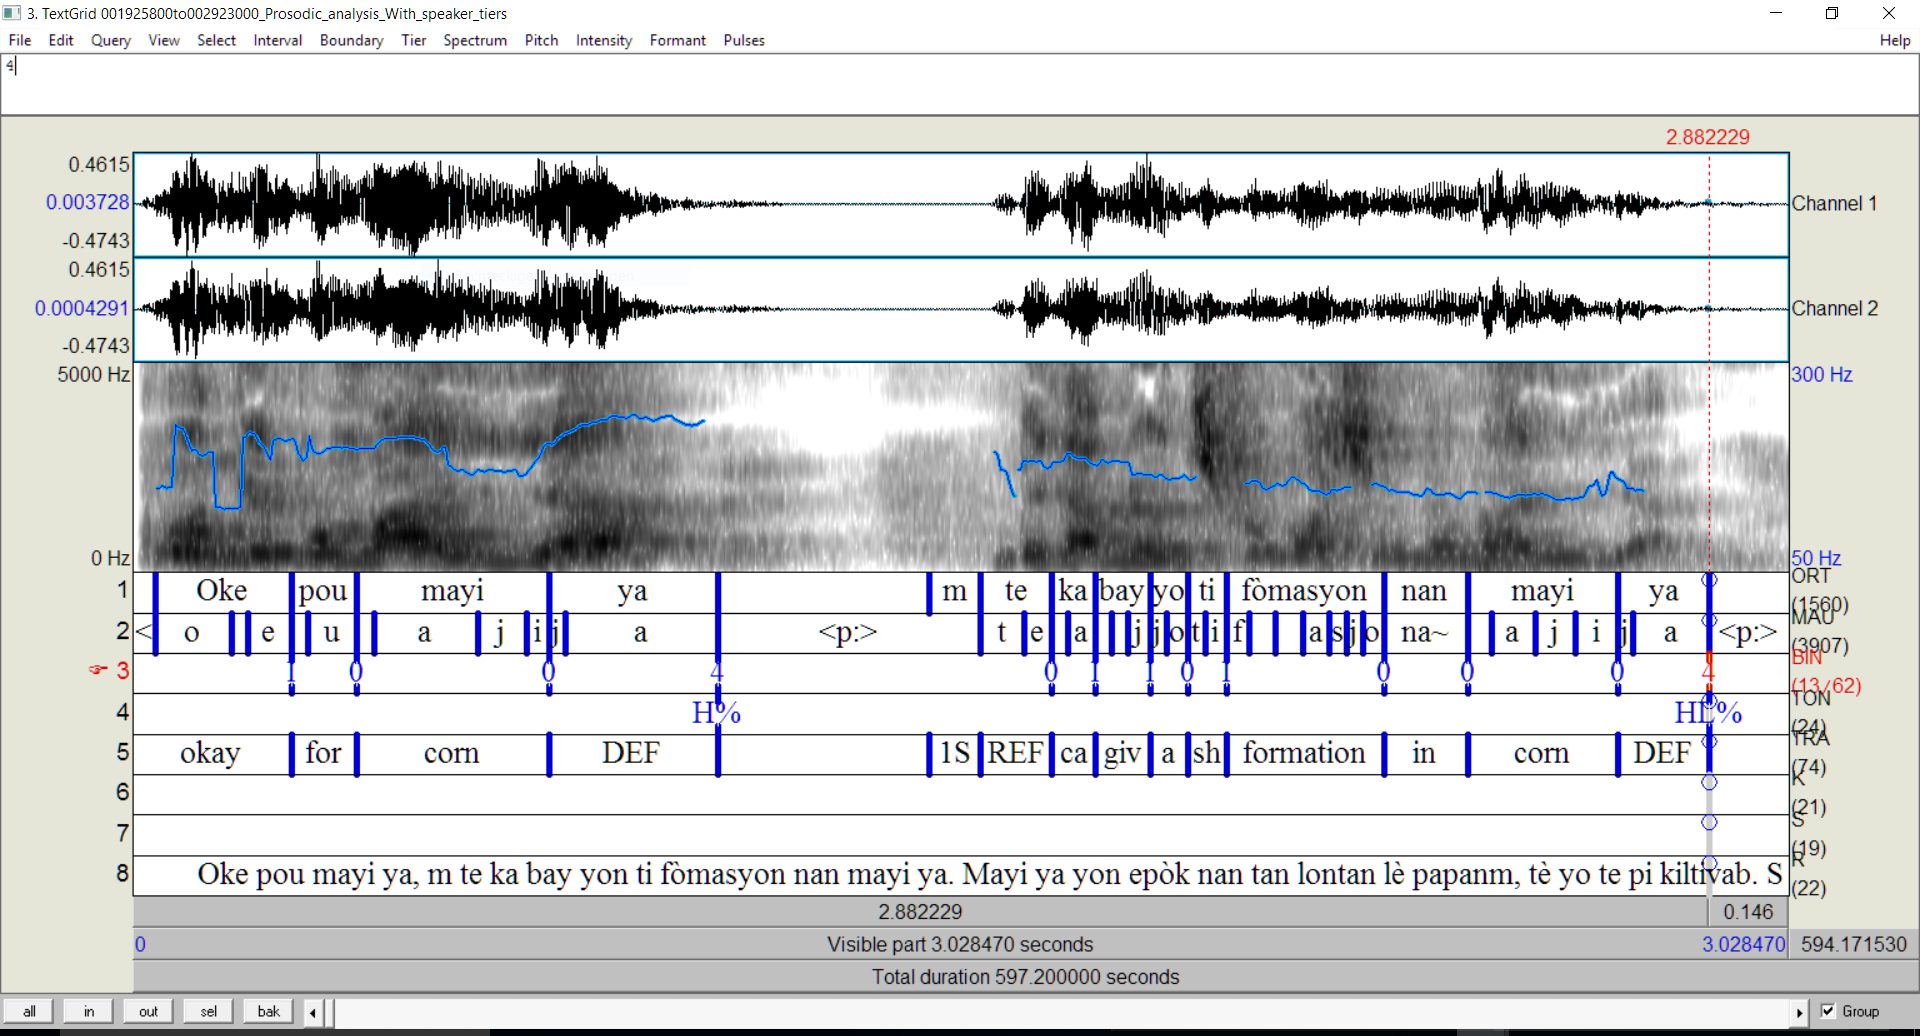
\includegraphics[width=\textwidth]{figures/KALPeerreviewedkorr-img3.png}
\caption{\label{fig:kal:3} Tier hierarchy and example of prosodic annotation.}
\end{figure}

\section{\label{sec:kal:4}Some prosodic features of Haitian Creole}

The linguistic interpretation of the annotated test piece allows some conclusions to be drawn about HC prosody. I sought empirical evidence for prosodic constituency, the location and phonetic nature of prosodic events within prosodic constituents, and salient tonal movements upon word classes. According to my working hypothesis of a hybrid prosodic system, I paid special attention to prosodic events on the right edge of prosodic constituents as a supposed influence of French and to tonal movements as a supposed influence of West African languages.

As mentioned above, I assume for HC the crosslinguistically attested prosodic structure of Intonational Phrase (IP) < Intermediate Phrase (ip) < Accentual Phrase/ clitic group (AP) < prosodic word (ω) (for the controversial discussion on the definition and empirical adequacy of prosodic constituents see amongst others \citealt{Nespor2007,Ladd2008,Frota2012}). I advocate an integrated view of prosodic structure and prosodic constituency that takes into account syntactic and phonological constraints, such as phrasal structure, rhythmic rules, and intonational phenomena. 

Let us consider an example taken from my ten-minute test piece, where a HC speaker talks about two different ways to plant corn, one involving putting five and another one involving putting three corn seeds into a hole in the soil. The IP and ip structure is the following:\footnote{This fragment corresponds to lines 220 to 222 of the transcript and to the time interval from 0:50 to 1:00 min of my test piece.}

\ea \label{ex:kal:1}
\glt {[}Yo konn plante mayi ya senk grenn nan tou{]}\textsubscript{IP} {[}{[}yo fouye tou mayi ya{]}\textsubscript{ip} {[}yo mete senk grenn mayi{]}\textsubscript{ip}{]}\textsubscript{IP} {[}{[}Men nou menm konnya{]}\textsubscript{ip} {[}nou vin pa gen sezon menm jan{]}\textsubscript{ip}{]}\textsubscript{IP} {[}nou plante mayi a twa grenn{]}\textsubscript{IP} {[}e nou vin plante a yon distans tou.{]}\textsubscript{IP}
\\
\glt \textit{‘They use to plant the corn with five seeds in a hole. They dig a hole for the corn. They put five corn seeds in it. But we ourselves use, (because) we do not have the seasons in the same way, we plant corn with three seeds, and we plant at a totally different distance.’}
\z


IPs represent intonationally self-contained and in most cases semantically coherent units, which we could describe syntactically as sentences or subunits of sentences. Intermediate Phrases (ip) are assumed as coherent subunits of morpho-syntactically complex constituents or structures, such as subjects or objects, which means that they are defined more syntactically than phonologically. In the HC test piece, I could observe rising-falling and rising pitch movements followed by a pause as right edge marks of IPs (for two examples see \figref{fig:kal:4}).\footnote{Please note that for the graphics in subsections 4, I removed the segment (MAU) and speaker tiers (K, S, R).} Of course, further research on boundary tones has to be done in the context of an intonational phonology of HC. Moreover, I want to point out that – in contrast to the rising-falling pitch movement – the rising right edge mark is realized in many cases upon the function word class \textsc{def} (definite article). Further remarks will follow below.

\begin{figure}  
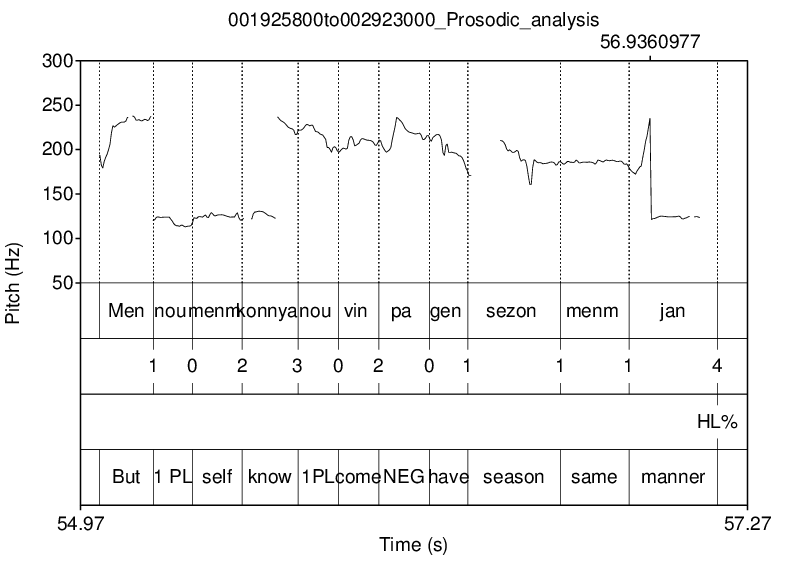
\includegraphics[width=.45\textwidth]{figures/KALPeerreviewedkorr-img4.png}
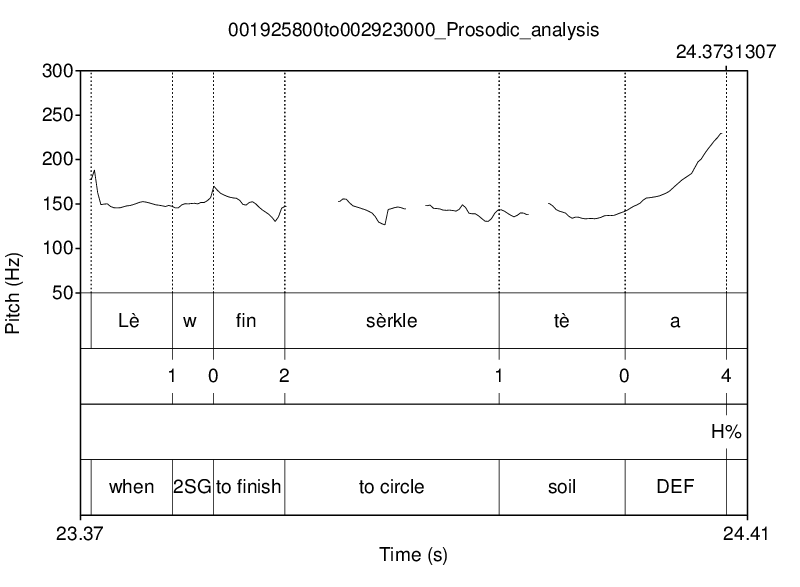
\includegraphics[width=.45\textwidth]{figures/KALPeerreviewedkorr-img5.png}
\caption{\label{fig:kal:4} Examples of a rising-falling (on the left: : Men nou menm konnya nou vin pa gen sezon menm jan ‘But we ourselves use, (because) we do not have the seasons in the same way’) and a rising pitch movement (on the right: Lè w fin sèrkle tè a ‘When you finished to circle the soil’) at the right edge of HC IPs.
}
\end{figure}


APs or clitic groups are built by one or more content words accompanied by their depending grammatical function words that form one single prosodic unit, such as [mayi ya]\textsubscript{AP} (corn \textsc{def}). Prosodic words are single accentuable words, such as [grenn]\textsubscript{ω} (seed). \REF{ex:kal:2} shows the internal structure of the second IP taken from \REF{ex:kal:1} with its APs/clitic groups and prosodic words:

\ea \label{ex:kal:2}
\gll [[[yo                       fouye]\textsubscript{AP} [tou]\textsubscript{ω} [mayi             ya]\textsubscript{AP}]\textsubscript{ip} [[yo  mete]\textsubscript{AP} [senk]\textsubscript{ω} [grenn]\textsubscript{ω} [mayi]\textsubscript{ω}]\textsubscript{ip}]\textsubscript{IP} 
\\
{\db}{\db}{\db}3.\textsc{pl}     dig                      {\db}hole          {\db}corn    \textsc{def}                    {\db}{\db}3\textsc{pl}  put                {\db}five                 {\db}seeds               {\db}corn
\\
\\
\textit{‘They dig a hole for the corn. They put five corn seeds in it.’}
\z

I argue that the most important prosodic domains for HC intonation/rhythm patterns are both the prosodic word and the AP/clitic group. The acoustic analysis indicates that intensity rises play a crucial role for producing prominences within non-IP-final prosodic words and AP/clitic groups. Those prominences can be classified as stress accents (see \citealt[3-53]{Hulstetal2010} for a discussion on word accent terminology). Pitch movements seem to be restricted to indicate IP boundaries. Moreover, the analysis clearly indicates that the mentioned prosodic events are located at the right edges of the HC prosodic constituents. Further prosodic research has to be done to specify the contribution of final lengthening and articulatory effort for the HC stress accent system.

The graphics in \figref{fig:kal:5} visualize the difference between intensity and pitch within one and the same IP. One can see that the intensity contour is much more eventful than the pitch contour, which stays quite flat across wide swathes of the IP. As we can see, there is an intensity peak on the vocalic part of the rightmost syllable of every prosodic word and AP/clitic group. Thus, the specific HC speech rhythm – especially compared to the French phrasal accent – results from the fact that every prosodic word and AP/clitic word have their own prominences produced by intensity rises and IP-final pitch movements on their right edges. 

\begin{figure}  
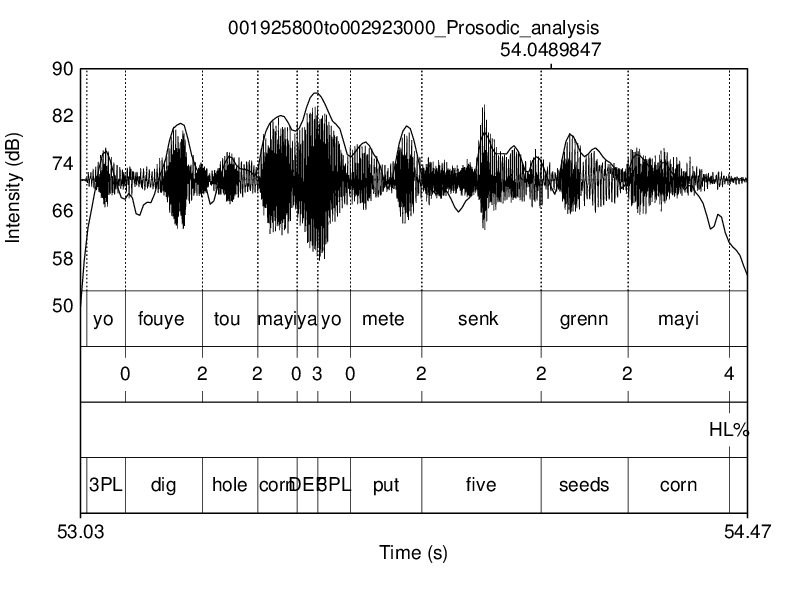
\includegraphics[width=\textwidth]{figures/KALPeerreviewedkorr-img6.png}
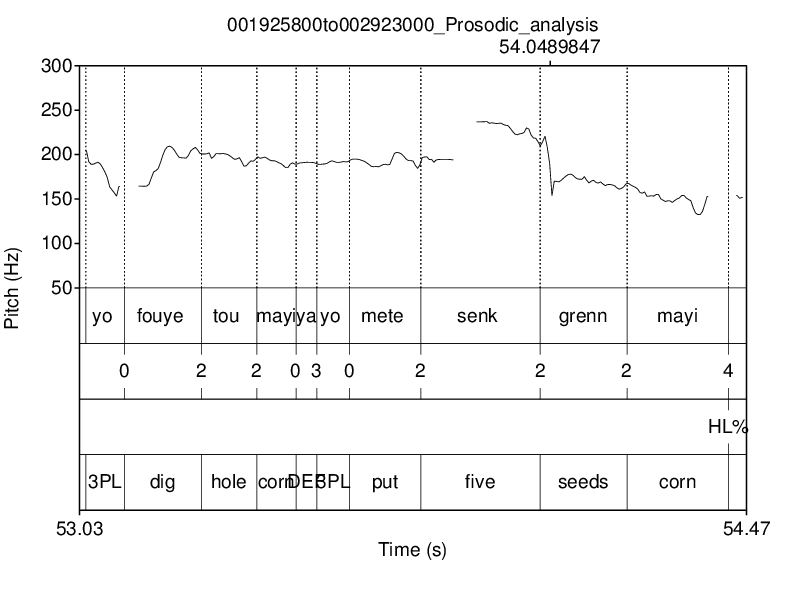
\includegraphics[width=\textwidth]{figures/KALPeerreviewedkorr-img7.png}

\caption{\label{fig:kal:5} Amplitude and intensity contour (on the left) and pitch contour (on the right) of the speech signal from the example in (2) \textit{yo fouye tou mayi ya yo mete senk grenn mayi} ‘They dig a hole for the corn. They put five corn seeds in it.’}
\end{figure}


As mentioned above, I observed a word-category-specific pitch movement upon the function word class \textsc{def} (definite article) within IP-final APs/clitic groups (for an example see <tè a> (soil \textsc{def}) on the right graphic in \figref{fig:kal:4}). \figref{fig:kal:6} and \figref{fig:kal:7} illustrate the IP-final and IP-non-final versions of the lexically identical structure \textit{mayi-ya} (corn \textsc{def}). As we can see, there is in both cases a prominence upon the definite marker \textit{ya}: in the IP-final version by means of intensity \textit{and} pitch rise and in the IP-non-final version by means of intensity rise while the pitch curve does not alter.

\begin{figure}  
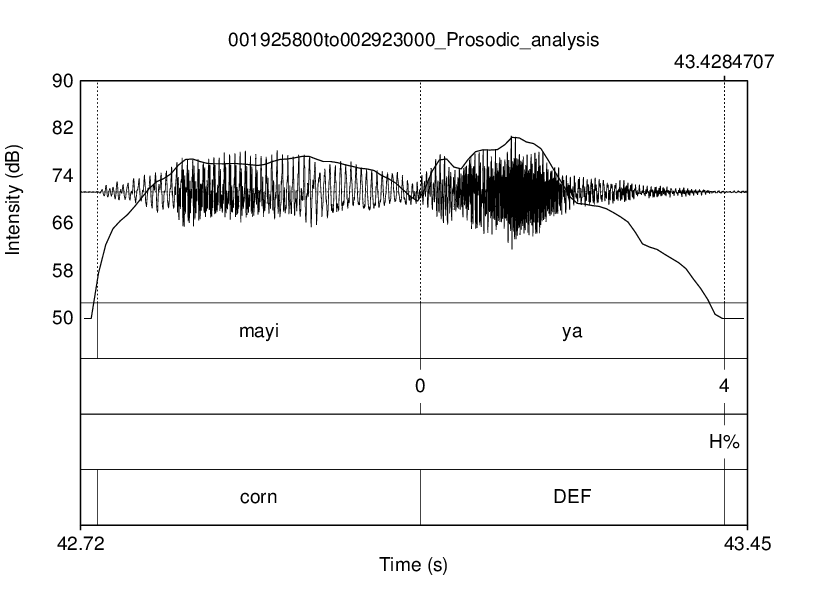
\includegraphics[width=\textwidth]{figures/KALPeerreviewedkorr-img8.png}   
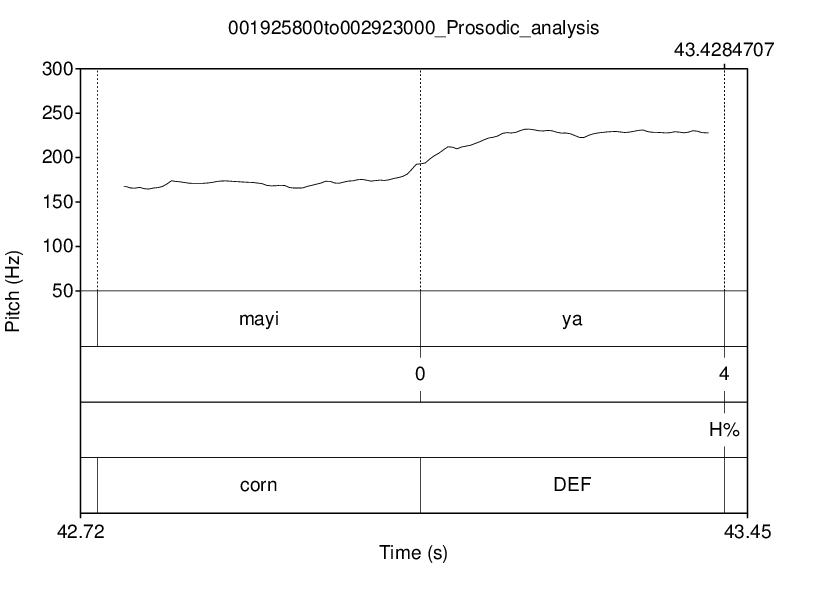
\includegraphics[width=\textwidth]{figures/KALPeerreviewedkorr-img9.png}
 
\caption{\label{fig:kal:6} Amplitude and intensity contour (on the left) and pitch contour (on the right) of IP-final prominence upon the word category \textsc{def} \textit{(definite article) mayi ya} ‘the corn’.}
\end{figure}

  
\begin{figure}
 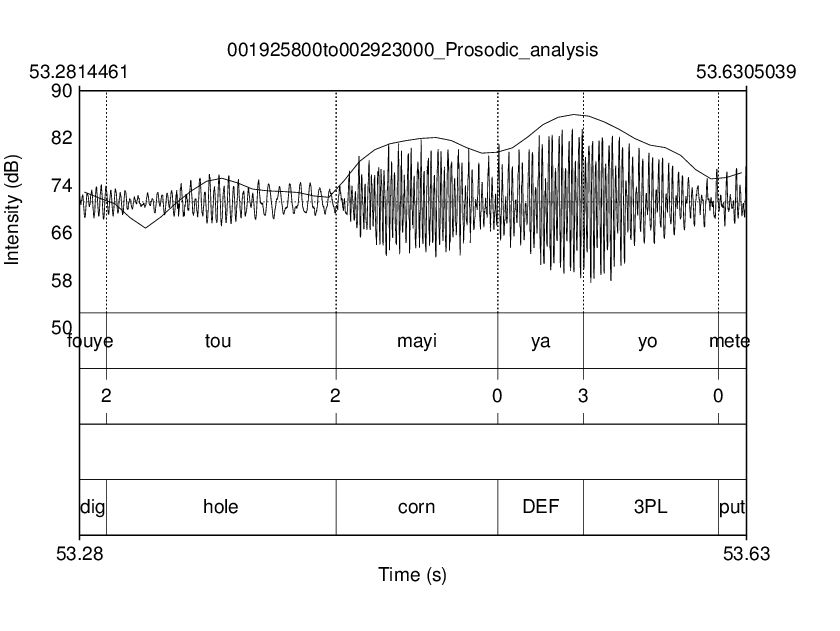
\includegraphics[width=\textwidth]{figures/KALPeerreviewedkorr-img10.png}   
   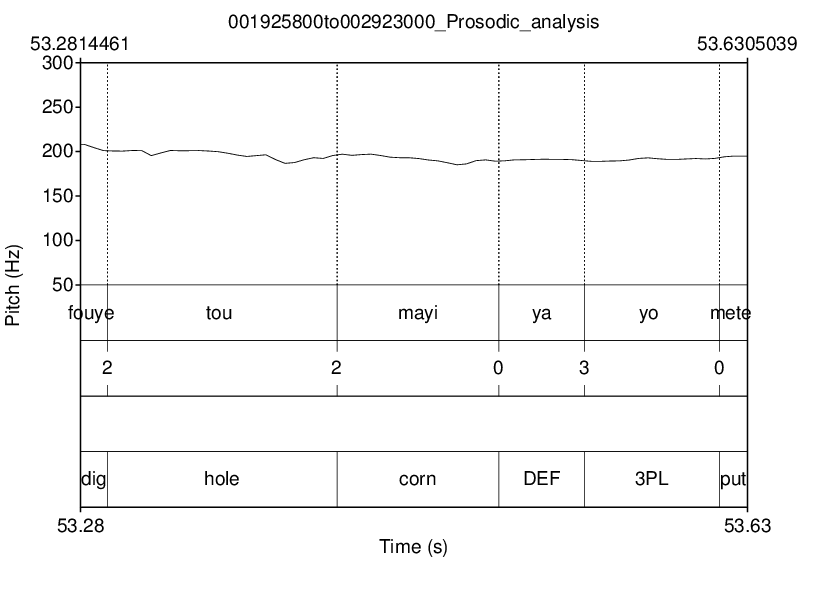
\includegraphics[width=\textwidth]{figures/KALPeerreviewedkorr-img11.png}
   
\caption{\label{fig:kal:7} Amplitude and intensity contour (on the left) and pitch contour (on the right) of IP-non-final prominence upon the word category \textsc{def} (definite article) from the example in (2) \textit{yo fouye tou mayi ya yo mete senk grenn mayi} ‘They dig a hole for the corn. They put five corn seeds in it.’}
\end{figure}


Here we can indeed identify an influence from West African grammatical and prosodic systems. The postpositive HC definiteness markers \textit{-la} with its phonetic alternations \textit{-a}, \textit{-an}, \textit{-nan}, -\textit{lan}, and \textit{-ya} for singular and -\textit{yo} for plural \citep[119-122]{Stein2017} are attributed to West African languages. For instance, the HC definiteness markers \textit{-la} and \textit{-a} are identical to the Ewe forms and in both languages, HC and Ewe, the plural definiteness marker is derived from the third person plural personal pronoun \citep[38]{Sylvain1979}. In addition to this formal identity, in Ewe those morphemes are prosodically marked by tonal movements or grammatical tones \citep[133-202]{Stahlke1971}. HC clearly does not have lexical tones, but it makes grammatical and information structuring use of prosodically marked prominences comparable to tones. The difference seems to be that HC speakers produce these prominences by means of pitch excursion only in IP-final contexts, while within IPs they increase intensity.


\section{\label{sec:kal:5}Remarks about the corpus-based approach to HC prosody and intonation}
Based on my experience with the handling of HC corpus data, I want to make the following remarks about the advantages and disadvantages of a corpus-based approach to prosody and intonation.

Currently, (spoken and written, synchronic and diachronic) creole language corpora are a prolific and quite quickly evolving field (see amongst others \citealt{Hagemeijer2014} for the building of a Gulf of Guinea Creole corpus and \citealt{Kriegel2015} for an overview of French-based creole corpora). Besides the \textit{Corpus of Northern Haitian Creole}, there are a few other online resources for spoken HC data of varying quality and functionality. The online \textit{Atlas of Pidgin and Creole Language Structures} \citep{Michaelis.apics} provides one short sample of HC with the following functionalities: audio–text alignment, glossing, translation into French, the transcript file and MP3 audio files are downloadable, Creative Commons license. The French meta-platform COCOON \citep{LACITO.cocoon} gives access to several recordings of spoken HC from the 1980s. The functionalities of this collection are the following: no audio–text alignment, no glossing, no translation into French, only the audio files are downloadable. To develop an automatic translation system, the Language Technologies Institute of Carnegie Mellon University’s School of Computer Science designed and built the \textit{Haitian Creole language data} corpus \citep{CMUSCS.haitiancreole}, which has the following functionalities: no audio–text alignment, no glossing, no translation into French or English, the WAV and TXT files are downloadable.

Drawn from my experience, the following functionalities are essential for further analytic usage of corpus data: audio–text alignment, glossing, translation, data download, license for data use and publishing, and clear indication for citation. The more of these functionalities are available, the easier the use for linguistic analysis is. Unfortunately, there is still no creole corpus that complies with all of these functionalities.

At first glance, there is one obvious advantage: (re)using existing speech data collections is economic and sustainable, especially if we consider language communities that live far from our own home country. Instead of prior resource-consuming (time, money, infrastructure) fieldwork and recordings, we can start with linguistic analysis nearly immediately.

Besides that undeniable merit, many technical and methodological problems arise while approaching and using corpus data. On the one hand, these are related to the general properties of linguistic corpora, which linguists usually create for specific research questions (see also \citeauthor{GarridoAlminana.2018}, this volume). In the case of the \textit{Corpus of Northern Haitian Creole}, linguists have explored the corpus data for lexical, morphophonological, syntactical, and sociolinguistic concerns (for recent research see, for example, \citealt{Valdman2015}). In this regard, the corpus reflects the creolistic research focus on lexis and grammar. Thus, the design of the interviews and the quality of the recordings did not pay special attention to the usability of the speech data for later phonetic, prosodic, or even intonational analyses. 

On the other hand, many problems of today’s usability have to do with technical standards, potentials, and limits of the date of origin of the corpus in question. For example, the audio files of the \textit{Corpus of Northern Haitian Creole}, recorded in 2007, have been saved in the MP3 audio format, which saves disk space but damages the audio signal. Today the memory capacity of electronic recording devices and of databases is usually not a problem anymore and audio data can be stored as large WAV files without limiting the field recordings and later website functionalities. If audio compression is needed for some reason, it should be executed by lossless compressed digital audio formats such as FLAC ({{F}}ree {{L}}ossless {{A}}udio {{C}}odec). Moreover, there is no alignment between the audio and the transcript files in our HC corpus – a fact that considerably hampered the use of the corpus data for phonetic analysis in Praat. Today, audio or multimedia data can be aligned and annotated quite easily with freely downloadable annotation software for spoken language such as ELAN \citep{Wittenburg2006} or EXMARaLDA \citep{Schmidt.2009}. Transcribers should use these computer programs instead of creating separate Word or Excel documents.

Another weak point of the recordings from the \textit{Corpus of Northern Haitian Creole} is that the different speakers of each interview, i.e. two test persons and the interviewer, are recorded on one single audio channel. Consequently, I had to chunk-segment the test piece for the MAUS segmentation procedure, a step that can be very time-consuming, especially in the case of large amounts of corpus data. Therefore, each speaker should be recorded on a separate audio channel or turn-segmented with the mentioned ELAN or EXMARaLDA annotation tools. 

A general challenge for corpus-based creole language prosody and intonation research are the background noises due to the natural environment of the interview settings such as crickets, barking dogs, human voices, and human activities such as playing children or the use of tools. Thus, only some parts of our HC corpus are usable for phonetic analysis. Hence, researchers in the field creating new corpus data should seek noise-reduced recording facilities.

The ten interviews of the \textit{Corpus of Northern Haitian Creole} are designed in a very similar way: In the presence of Albert Valdman, a local teacher conducts the conversation about different topics, such as agriculture, traditions, festivities, working activities, and so on, of two native speakers of the Northern HC variety. A major methodological problem for HC intonation research is that the researcher has to content him/herself with the speech data from the corpus. There are no speech data from pragmatically controlled elicitation of particular illocutionary acts, such as statements, exclamatives, yes/no-questions, wh-questions, imperatives, vocatives, or enumerations, by means of Discourse Completion Tasks (\citealt{Prieto.2001,Prieto2010,Jun2014,frotaPrieto2015,Prieto2010.2014.Atlas}, \citeauthor{Vanrell.2018}, this volume). Nevertheless, as the enumeration pattern in \REF{ex:kal:3} shows, contextually embedded intonational patterns can be found within the corpus. Here the non-final elements \textit{fevriye} 'February' and \textit{mas} 'March' are realized with a rising LH tonal movement and the final element of the enumeration \textit{avril} 'April' is realized with a rising-falling tonal movement L+HL. However, this inductive, yet knowledge-driven, approach to illocution needs deeper methodological consideration, e.g. by comparing elicitated tonal patterns with contextually embedded ones of the same illocutionary act.


\ea\label{ex:kal:3}
\gll nou      plante             mayi  fevriye …   nou          plante             mayi  mas\\
1\textsc{pl}  plant\textsc{pst}  corn  February …  1\textsc{pl}  plant\textsc{pst}  corn  March\\
\\
\textit{'We planted corn in February, we planted corn in March,}\\
\gll nou  plante  mayi … avril\\
1\textsc{pl}  plant\textsc{pst}  corn … April\\
\\
\textit{we planted corn in April'}\\
\z


To sum up this section, I would like to say that for the moment a corpus-based approach to HC prosody and intonation is much more practicable for the former. User-friendly data-driven intonation research still remains a desideratum. Of course, there are (highly idiosyncratic) automatic parametric data-driven approaches to intonation (\citealt{Moehler1998,Taylor2000,Reichel2010,Reichel.2014}, see there for related references), which are promising for the future for exploring corpus data.

\section{\label{sec:kal:6}Conclusion}
The goal of the investigation in hand was to assess the potentials and limits of a corpus-based approach to HC prosody. Hence, my main concern was the fitting of speech data taken from the existing online \textit{Corpus of Northern Haitian Creole} for prosodic analysis in Praat. Starting with separately saved audio and transcript corpus files, I successfully established a workflow for the audio–text alignment and a word- and phoneme-sized segmentation of a ten-minute test piece by using BAS tools from the CLARIN-D research infrastructure. The Praat text grids thus obtained could be merged and used for commonly used prosodic analysis procedures in Praat. Moreover, those analyses revealed several preliminary facts concerning HC prosody.

In summary, my corpus-based approach to HC prosody remains only a first, but promising, step toward a broader picture of the topic. In any case, creolists can explore a large amount of already existing corpus data. Further research has to be done for example on duration patterns, such as final lengthening within HC prosodic constituents, and on the systematic relationship between pitch movements and intensity rises to generate prominences. 

Overall, the hybrid system hypothesis is an illuminative approach to creole grammar genesis \citep{Aboh2015} as well as to prosody and intonation (\citealt{Brousseau2003,Gooden2009}), which goes hand in hand with the perception-based idea of the filter function of the African substrate languages while interpreting lexifier language structures and features during uncontrolled language acquisition (\citealt{Hazael-Massieux1993}). The observed HC prominence pattern upon the word category \textsc{def} within the syntactic structure of noun-\textsc{def} might be an illustrative example.

\section{References}

\section*{Acknowledgements}

I am very grateful to Uwe Reichel from the Ludwig Maximilian University of Munich who accompanied this process to enable the use of the BAS tools for Haitian Creole alignment and segmentation.

{\sloppy
\printbibliography[heading=subbibliography,notkeyword=this]
}

\end{document}